%!TEX root = main.tex
\chapter{Camera Models and Calibration}

Computer vision works much like the same way human vision works. Light rays
emitted from a light source, such as a lamp or the sun, travels until it hits
an object. Depending on the objects physical properties (light absorption,
reflection and emission spectra), the light re-emitted by that object that
eventually reaches our eyes determines which color we perceive the object has.

A camera is very similar to our eyes; in place of the eyes cornea and lens,
iris and retina, a camera has glass lenses, aperture and imager respectively.
There are of course differences, like the retina resting on a curved,
spherical surface, while an imager being a flat squared plane, the camera
lenses are moved to focus, while the eyes lenses changes shape. But none of
this really matters; what is most important is the geometry of the arrangement
of the components. The geometry and, especially, ray tracing mathematics plays
a large role in computer vision.

This chapter will briefly explain how a camera works, camera intrinsic and
extrinsic matrices, and how the images must be prepared before continuing down
the depth estimation pipeline. For more exhaustive information on these
topics, refer to \emph{O'reilly Learning OpenCV}\ref{open-cv}.

\section{Pinhole Camera Model}

The simplest model is the \textit{Pinhole camera model}. The model describes
the mathematical relationship between the coordinates of a 3D point and its 2D
projection onto the image plane. An ideal pinhole camera is one where the
pinhole only lets inn a single light ray from any point in the scene.  An
example of pinhole a camera is shown in figure \ref{fig:pinhole-camera-model}.

\begin{figure}[h]
  \centering
  \label{fig:pinhole-camera-model}
  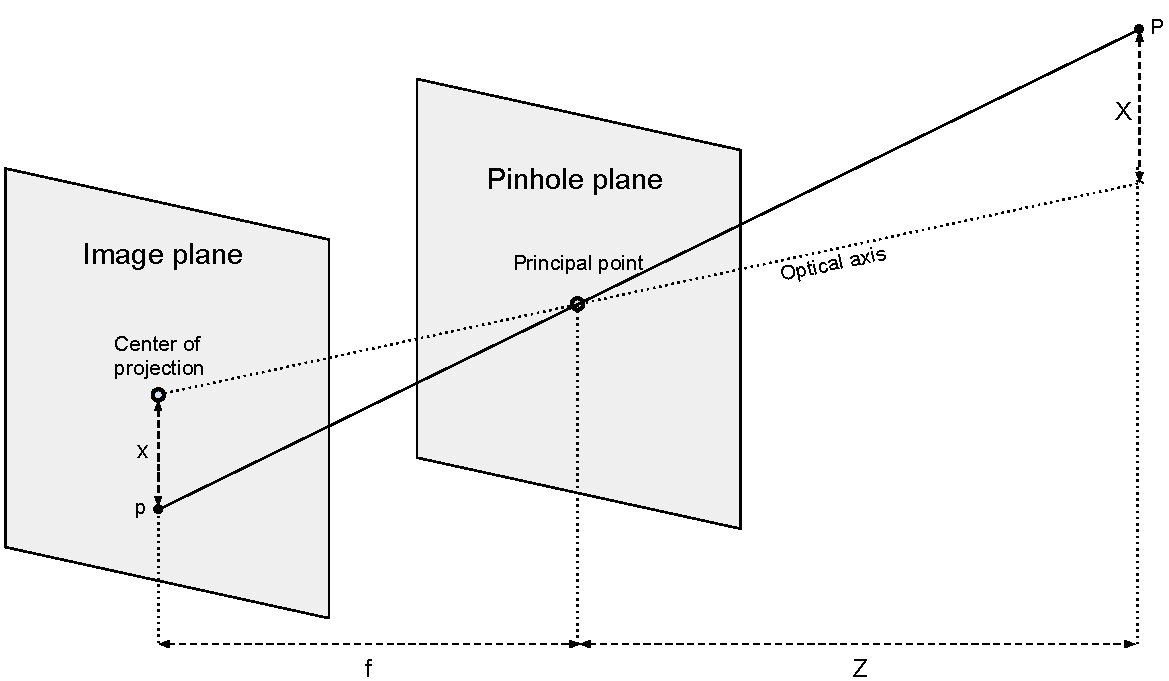
\includegraphics[width=\textwidth]{images/Pinhole-camera-model.pdf}
  \caption{A diagram of a pinhole camera showing the important features of the model}
\end{figure}

The \emph{principle point} is the pinhole itself, the point which all the rays
projected into the \emph{image plane} intersect. The \emph{optical axis} is
the axis perpendicular to the image plane that intersects the principle point,
and the \emph{center of projection} is where the optical axis intersects the
image plane. \emph{X} (capital X) is the distance between a point \emph{P} in
the 3D scene and the optical axis, and \emph{x} is the distance between
projected point \emph{p} and the center of projection. \emph{f} is the focal
length, the distance between the principle point and the center of projection,
and \emph{Z} is the distance from the principle point to the point P in the 3D
scene.

\begin{figure}[h]
  \centering
  \label{fig:rearranged-pinhole-camera-model}
  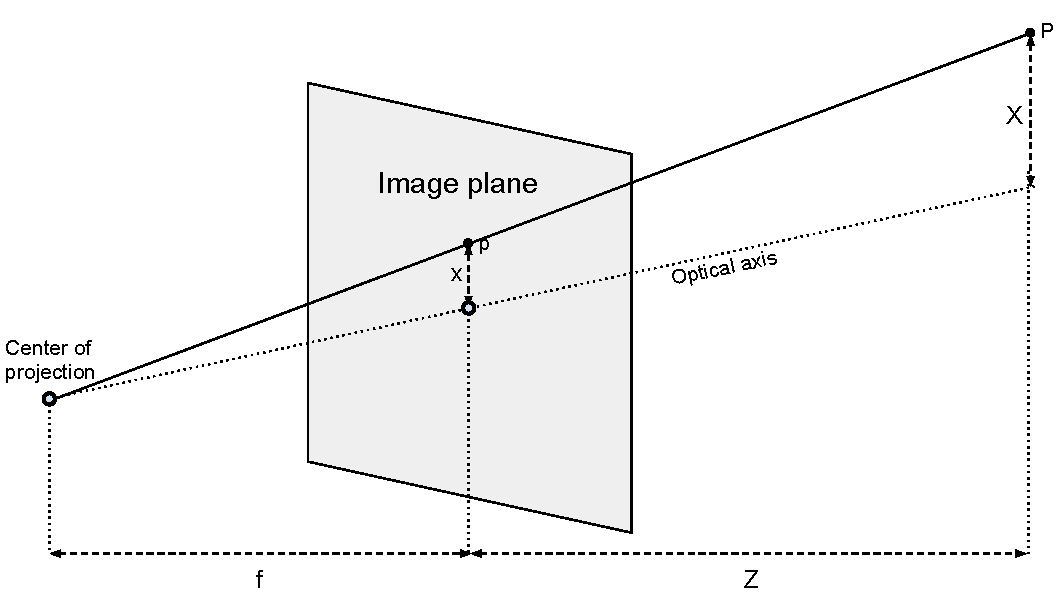
\includegraphics[width=\textwidth]{images/rearranged-Pinhole-camera-model.pdf}
  \caption{A diagram of a pinhole camera showing the important features of the model}
\end{figure}

As can be seen in the figure, we can use similar triangles to get $-x =
f\frac{X}{Z}$. To make the math easier, the model is usually rearranged such
that the image and pinhole planes, shown in figure \ref{fig:rearranged-
pinhole-camera-model}. In this arrangement, the pinhole is now the center of
projection, the point which all rays travel towards. The image created by rays
intersecting the image plane is equivalent to the image created in the
previous model, but it is no longer upside down. The similar triangles
relationship $x = f\frac{X}{Z}$ is now more evident.




It is a simple model, so it does not take into account geometric distortions
or blurring of unfocused points.

Distortions:
    lens barrel
    color
    brightness



\section{Calibration}

\subsection{Basic Projective Geometry}

\section{Lens Distortion}

